
\chapter{\textsf{Central Management}}

The main frame of Central Management consists in four areas:

\begin{description}
	\item[Top panel -] This panel provides the necessary menus for main system configuration, such as user administration, ISOs management and the interface that shows the system events.
	\item[Left panel (\emph{Nodes}) -] This panel lists the real machines/virtualization servers - {\bf\emph{nodes}} - and any existing virtual machines - {\bf\emph{servers}}. The first level of the tree show the system datacenters. After that level we can find the available physical servers, and on the bottom nodes the virtual machines. All functionalities that can be donne on each node of the tree, are described on Section \ref{sec:node}(Node) and in Section \ref{sec:server}(Server). When some node is clicked, its information is loaded and appears on the main panel.
	\item[Main panel (at right) -] In this area is displayed the information about the selected node.
	\item[Information panel (at bottom) -] This areas shows the volatile information about any operations made on the interface. Here we can found the success of the operations.
\end{description}

\opt{etvm}{
 \begin{figure}[H]
    \begin{center}
   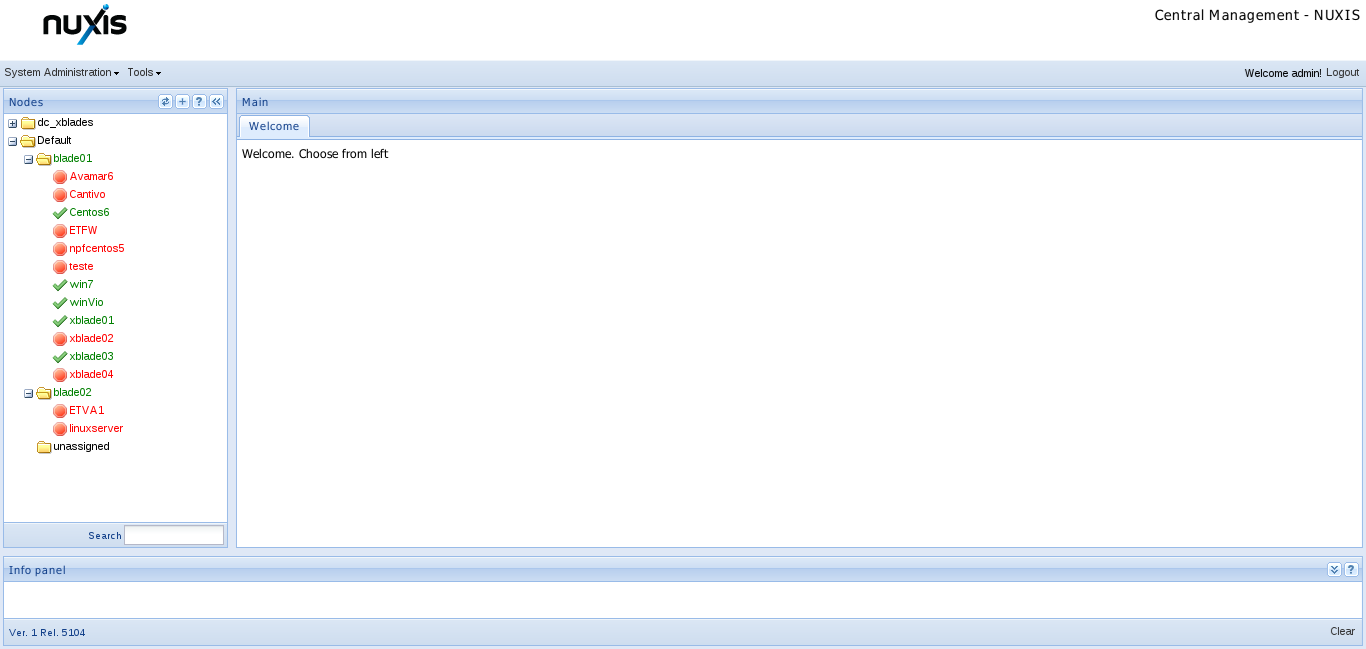
\includegraphics[scale=0.45]{screenshots/principal_nuxis.png}
   \caption{Layout principal}
   \label{fig:principal}
   \end{center}
\end{figure}
}
\opt{etva}{
\begin{figure}[H]
   \begin{center}
    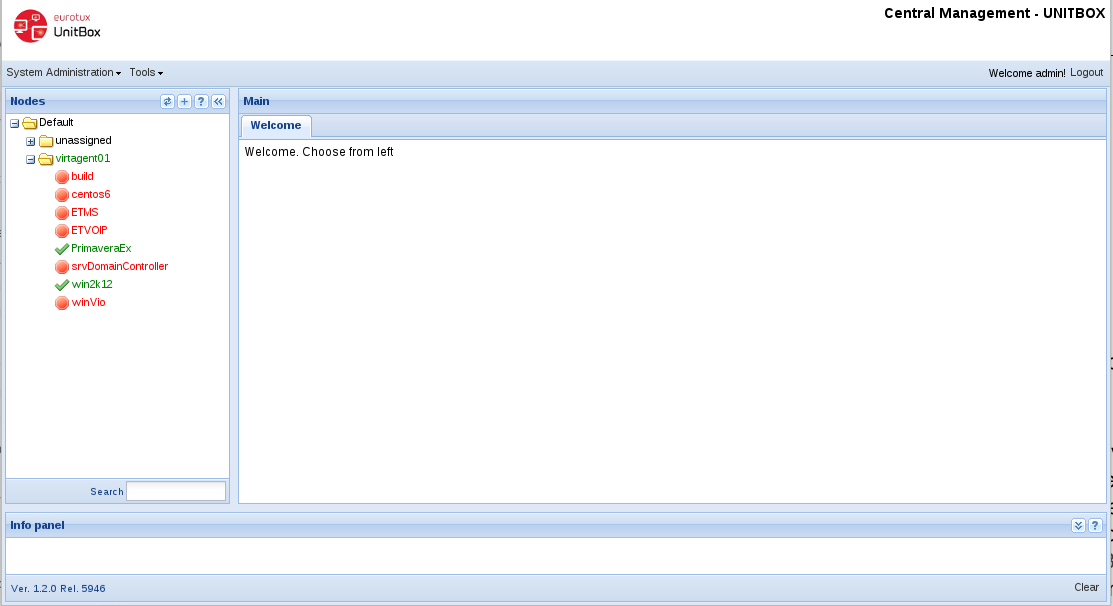
\includegraphics[scale=0.45]{screenshots/principal.png}
    \caption{Layout principal}
    \label{fig:principal}
    \end{center}
 \end{figure}
}

\pagebreak


\section{First access}
\label{sec:first_access}
After the installation, the CM can be accessed on the web browser by entering the address http://<IP ADDRESS>\footnote{The ip address is specified during the installation process\opt{etva}{
 , described in Chapter \ref{chp:installation}}
.}

\opt{etvm}{
    \begin{figure}[H]
    \begin{center}
    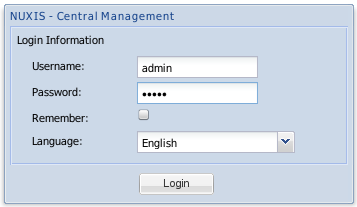
\includegraphics[scale=0.7]{screenshots/login_nuxis.png}
    \caption{Authentication window}
    \label{fig:login}
    \end{center}
    \end{figure}
}
\opt{etva}{
    \begin{figure}[H]
    \begin{center}
    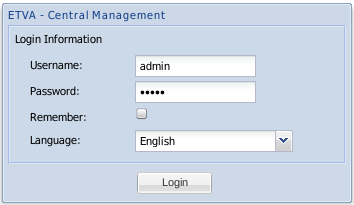
\includegraphics[scale=0.7]{screenshots/login_etva.png}
    \caption{Authentication window}
    \label{fig:login}
    \end{center}
    \end{figure}
}

The Figure \ref{fig:login} shows the first displayed frame, that asks the user his username and password. In this window we can also select the pretended language\footnote{Currently two languages are available: Portuguese an English}.

\begin{quote}
	{\large \bf Note} \\*[-.8pc]
	\underline{\hspace{6in}} \\
    The default credentials are:
	\begin{description}
        	\item[Username:] admin
	        \item[Password:] admin
	\end{description}
    For safety reasons the default password should by changed. This can be donne after the first access, on the \textit{first time wizard}.

\end{quote}

During the first access, the user is prompted with some questions, that allows him to setup the system (see Section \ref{sec:first_time_wizard}).

After the installation and configuration of the CM, and having an already installed agent, it should appear automatically on the left panel.

On the left panel, see Figure \ref{fig:principal}, will appear the virtualization \emph{node} registered on CM. We can right click the \emph{node} and select the option \emph{Authorize}. In this case the cm sends a message to the virtualization agent, requesting information about the \emph{node}. After the end of the authorization process, the \emph{node} can be managed as stated on Section \ref{sec:node}.

\pagebreak

\section{Default cluster}

%In the Main tab 
In this panel we can see an overview of the CM. The virtualization servers can be seen as well as any existing networks (see Figure \ref{fig:main_nodes}).

\subsection{Nodes}
\label{sub:nodes}

In \emph{Nodes} we can see some information about the virtualization servers such as the supported hypervisor, the state of the virtualization server, among other info.

\begin{figure}[H]
	\begin{center}
	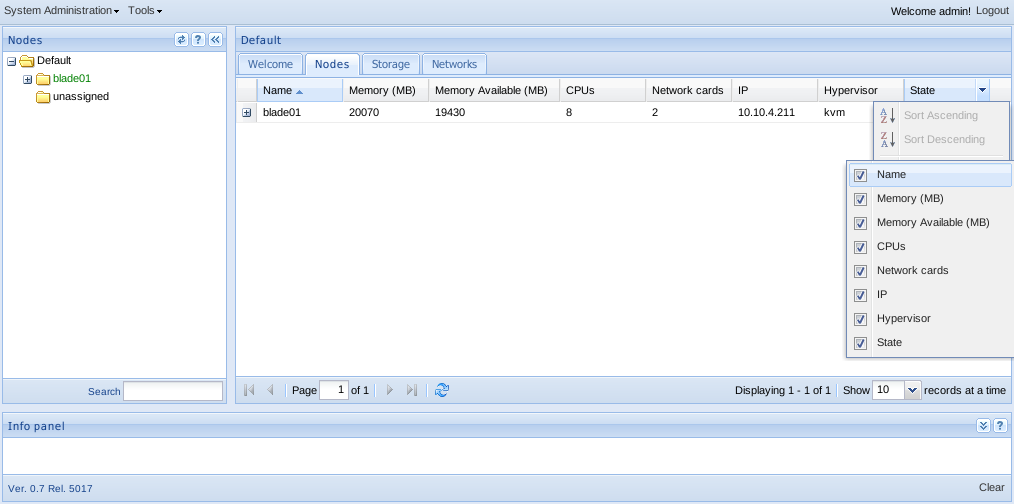
\includegraphics[scale=0.45]{screenshots/main_nodes.png}
	\caption{Central Management nodes view}
	\label{fig:main_nodes}
	\end{center}
\end{figure}

\subsection{Networks}
\label{sub:network}

This panel allow us to do the following operations:

\begin{itemize}
    \item System's network administration
    \item MAC address pool management
    \item Manage the virtual machines' network interfaces
\end{itemize}

\begin{figure}[H]
	\begin{center}
	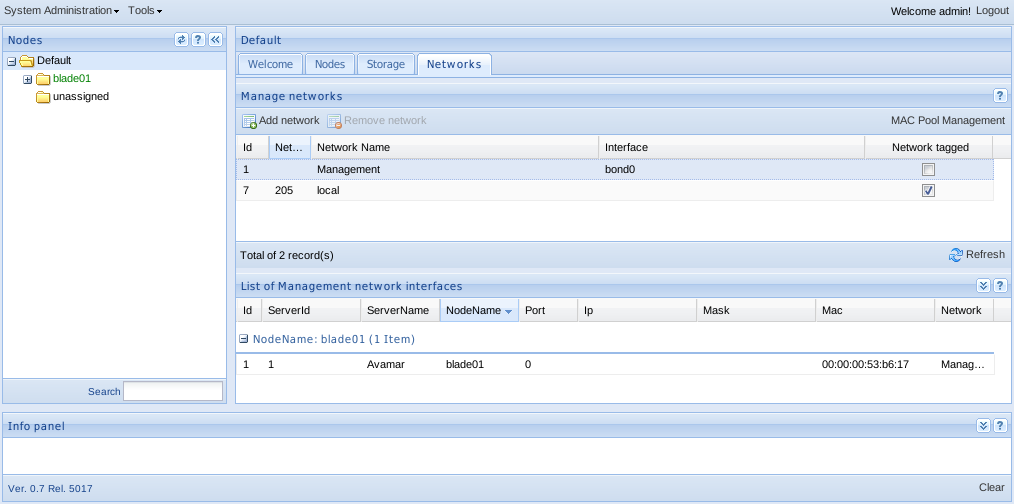
\includegraphics[scale=0.45]{screenshots/main_networks.png}
	\caption{System networks view and virtual machines' interfaces}
	\label{fig:main_networks}
	\end{center}
\end{figure}

Also, it's possible to filter the network interfaces by a given network, as stated on Figure \ref{fig:main_networks}.
The Figure \ref{fig:main_networks} lists the network interfaces for the network \emph{Internet}.

\subsubsection{Network administration}

To add a network, click on the \emph{Add network} button.

The network info is constituted by its name and ID\footnote{If the network/vlan is \emph{tagged}, the field \emph{network ID} refers to its \emph{VLAN ID} (see Figure \ref{fig:network_create})}

To remove a network, choose the desired network and press the button \emph{Remove network}. 

\begin{quote}
	{\large \bf Note} \\*[-.8pc]
	\underline{\hspace{6in}} \\
    The add/remove operations are only available on version \acronym.
\end{quote}


\begin{figure}[H]
	\begin{center}
	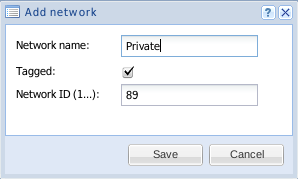
\includegraphics[scale=0.5]{screenshots/network_create.png}
	\caption{Add network window}
	\label{fig:network_create}
	\end{center}
\end{figure}

After successfully add or remove a network, all Central Management nodes are notified.

\subsubsection{MAC address pool management}
\label{sec:mac_pool}

On \emph{MAC Pool Management} (see Figure \ref{fig:main_networks}), its possible to create new addresses.
Also, we can see the associated network for each MAC address, and the available addresses.

\begin{figure}[H]
	\begin{center}
	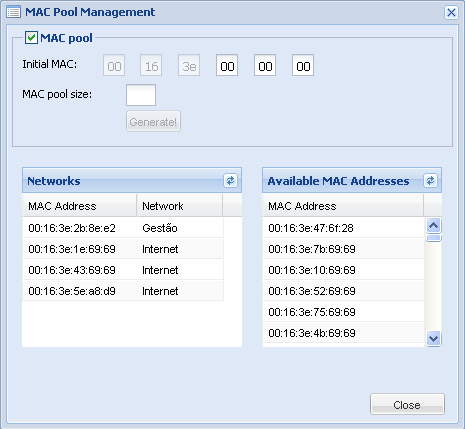
\includegraphics[scale=0.5]{screenshots/networks_macpool.png}
	\caption{MAC pool creation window}
	\label{fig:networks_macpool}
	\end{center}
\end{figure}


\subsubsection{Virtual machines' network interfaces management}
If we select a network interface and access to the context menu, it's possible to remove the network interface associated to this record - \emph{Remove network interface} or change the network interfaces for the associated virtual machine - \emph{Manage network interfaces}.

\begin{figure}[H]
	\begin{center}
	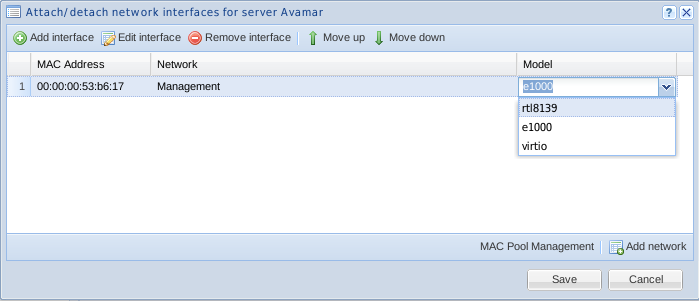
\includegraphics[scale=0.5]{screenshots/nics.png}
	\caption{Virtual machine interfaces (management window)}
	\label{fig:nics}
	\end{center}
\end{figure}

On the management window it's possible to select the network card's driver\footnote{This option is available on HVM or KVM machines. The available drivers are: e1000, rtl8139 e virtio}.

\section{Virtual cluster}
\label{sec:cluster}

On left side panel it's possible to select a \emph{cluster}(virtual cluster) and do the following operations:

\begin{itemize}
    \item \emph{Nodes} - View information about nodes (see Section \ref{sub:nodes})
    \item Storage - Storage management on \emph{Cluster} context (see Section \ref{sec:storage})
    \item Networks - Network management (see Section \ref{sub:network})
\end{itemize}

In addition. it's possible to access the context menu (right click) to perform the following operations:
\begin{itemize}
    \item Edit cluster
    \item Remove cluster
\end{itemize}

In \emph{Edit cluster} it's possible to change the name of \emph{cluster} and allow use to activate nodes high availability.
\begin{figure}[H]
       \begin{center}
       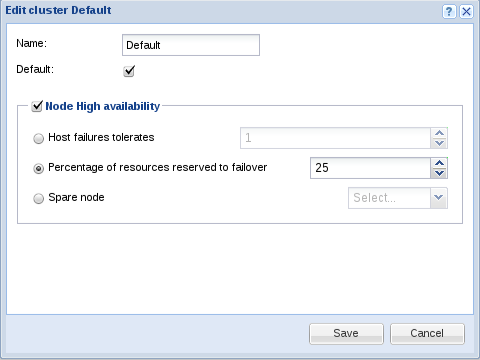
\includegraphics[scale=0.5]{screenshots/cluster_edit.png}
       \caption{Edit cluster}
       \label{fig:cluster_edit}
       \end{center}
\end{figure}

When we enable \emph{Node High availability}\footnote{The option \emph{Node High availability} will be enable only if \emph{fencing} configuration is defined for all node (see \ref{para:node_fencing_config})}, we may choose one of this options:

\begin{itemize}
    \item \emph{Host failures tolerates} - number of hosts in failure that we can garantee high availability with restrictions of resources allocation;
    \item \emph{Percentage of resources reserved to failover} - percentage of resources reserved to garantee the high availability of critical services;
    \item \emph{Spare node} - it's define one \emph{spare node} that will be used to garantee the high availability of one of the others nodes. This \emph{spare node} should have necessary resources to ensure the availability of critical virtual servers of fail node.
\end{itemize}

The \emph{Node High availability} provides, in failure case, the migration of the virtual servers by priority order (see figure \ref{fig:server_edit_ha}), to keep the services of this virtual servers operational.

The operation \emph{Remove cluster} removes information related to \emph{cluster} (nodes, networks and storage) from the \emph{Central Management} database.

% PAINEL NODE

\section{Virtualization server}
\label{sec:node}

On panel \emph{Nodes} it's possible to select a \emph{node}(virtualization server), and do the following operations:
\begin{itemize}
    \item See the \emph{node} information (see Section \ref{sec:nodeinfo})
    \item Manage its virtual machines (see Section \ref{sec:servers})
    \item Manage \emph{node} storage (see Section  \ref{sec:storage})
\end{itemize}

In addition to these options, it's possible to access the context menu (right click). This menu allow us to perform the following operations:
\begin{itemize}
    \item Load node
    \item Edit node
    \item Remove node
    \item Connectivity options \footnote{Only available on version \emph{NUXIS}}
    \item Change keymap
    \item Check node state
\end{itemize}

In \emph{Load node}, it's send one request to \emph{Central Management} for node state update.

For operation \emph{Edit node} it's available edition of server virtualization proprieties like name and \emph{fencing} device configuration.
\begin{figure}[H]
       \begin{center}
       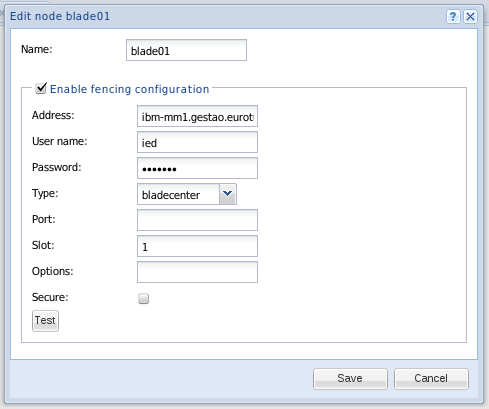
\includegraphics[scale=0.5]{screenshots/node_edit.png}
       \caption{Edit node}
       \label{fig:node_edit}
       \end{center}
\end{figure}
\label{para:node_fencing_config}In \emph{Enable \emph{fencing} configuration} we can activate \emph{fencing} device for node management and configure the parameters accord on following types: \emph{bladecenter}, \emph{virsh}, \emph{ilo}, \emph{ipmilan} e \emph{rsa}.

The operation \emph{Remove node} removes one node from the \emph{Central Management} and delete the information related to it on database.

In \emph{Connectivity options}, it's possible to configure the interface \emph{Management} that is connected with the virtualization agent. 
\begin{figure}[H]
	\begin{center}
	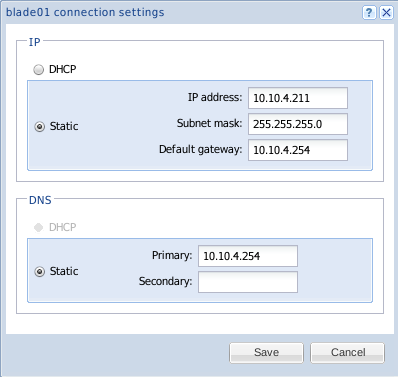
\includegraphics[scale=0.5]{screenshots/node_conn.png}
	\caption{Agent connectivity configuration}
	\label{fig:node_conn}
	\end{center}
\end{figure}

In \emph{Change keymap}, depending on the selected item, the virtualization server or virtual machine, it's possible to define the standard VNC keymap, or the specific virtual machine keymap.

In \emph{Node status}, it's possible to access to subset of options:
\begin{itemize}
    \item Check status - it send an request to the virtualization server to check the agent connectivity
    \item Maintenance / Recover - Put the node in maintenance/recover mode
    \item Shutdown - it shuts node down (see Section \ref{sub:shutdown_node}).
\end{itemize}

In operation \emph{Maintenance} we able to put node in maintenance mode in order to run maintenance tasks.
\begin{figure}[H]
   \begin{center}
   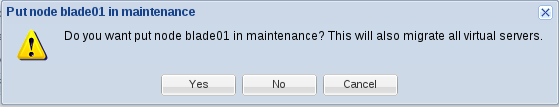
\includegraphics[scale=0.45]{screenshots/node_maintenance.png}
   \caption{Node maintenance}
   \label{fig:node_maintenance}
   \end{center}
\end{figure}
When node is moved to maintenance mode, the virtual servers will be migrated by priority order (see figure \ref{fig:server_edit_ha}).

The operation \emph{Recover} runs some tasks like node agent status check, connectivity and storage info consistency, before recover node from maintenance mode.

\subsection{Node information}
\label{sec:nodeinfo}
In \emph{Node information} we can see the information about the virtualization server. We can see the "real" machine supported hypervisors and, among other information, the virtualization agent's state.

\begin{figure}[H]
	\begin{center}
	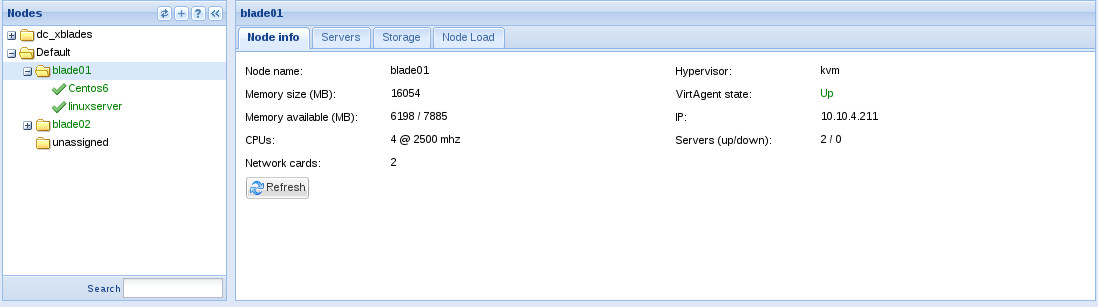
\includegraphics[scale=0.45]{screenshots/node_info.png}
	\caption{Node's information}
	\label{fig:node_info}
	\end{center}
\end{figure}

\subsection{Servers}
\label{sec:servers}
In \emph{Servers} we can see the information of every virtual machines existing on the selected virtualization server. In addition, allows to perform the following operations:

\begin{itemize}
	\item Add a virtual machine
    \item Edit a virtual machine
	\item Remove virtual machine
	\item Access virtual machine in a VNC console
	\item Start/Stop virtual machine
    \item Migrate virtual machine
    \item Snapshots
\end{itemize}
\begin{figure}[H]
	\begin{center}
	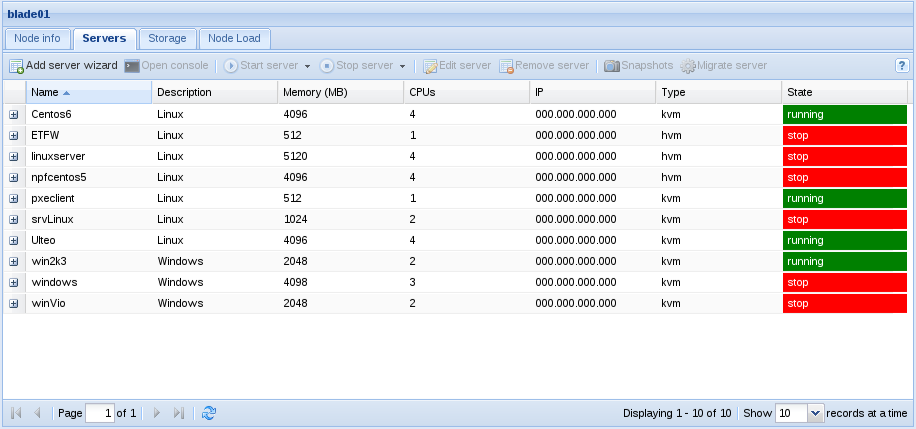
\includegraphics[scale=0.45]{screenshots/node_servers.png}
	\caption{Node's virtual machines}
	\label{fig:node_servers}
	\end{center}
\end{figure}

\subsubsection{Add virtual machine}
\label{sec:add_server}

To add a new virtual machine, press the button \emph{Add server wizard}.
\begin{quote}
	{\large \bf Note} \\*[-.8pc]
	\underline{\hspace{6in}} \\
    The panel options will be enable, if the virtualization agent is running on the \emph{node} (physical machine) and if it is able to stablish a connection with the CM.
\end{quote}
 

\begin{figure}[H]
	\begin{center}
	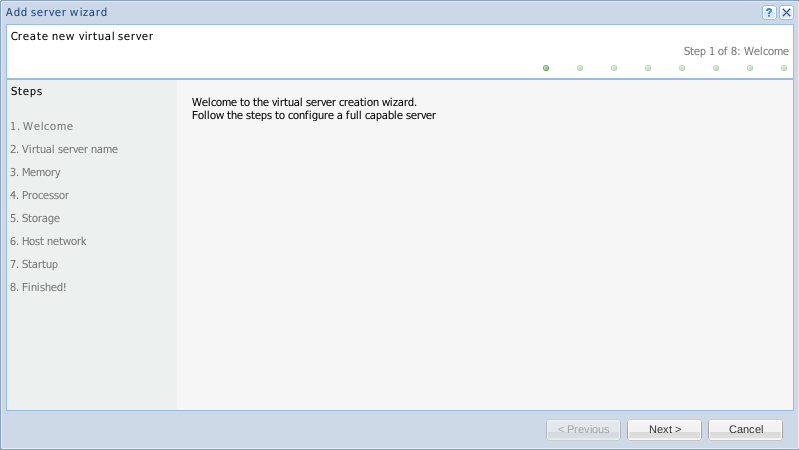
\includegraphics[scale=0.5]{screenshots/server_createwiz.png}
	\caption{Add server wizard - Welcome}
	\label{fig:server_createwiz}
	\end{center}
\end{figure}
The server wizard has the following steps:
\begin{description}
	\item[Virtual machine name:] In this step we can define the virtual machine name and the type of the operating system. The operating system option varies depending on the type of virtualization node.
		\begin{itemize}
			\item with XEN e hardware virtualization support:
			\begin{itemize}
				\item Linux PV
				\item Linux HVM
				\item Windows
			\end{itemize}
 			\item with XEN without hardware virtualization support:
			\begin{itemize}
				\item Linux PV
			\end{itemize}
 			\item with KVM
			\begin{itemize}
				\item Linux
				\item Windows
			\end{itemize}
		\end{itemize}
	
		\begin{figure}[H]
        		\begin{center}
		        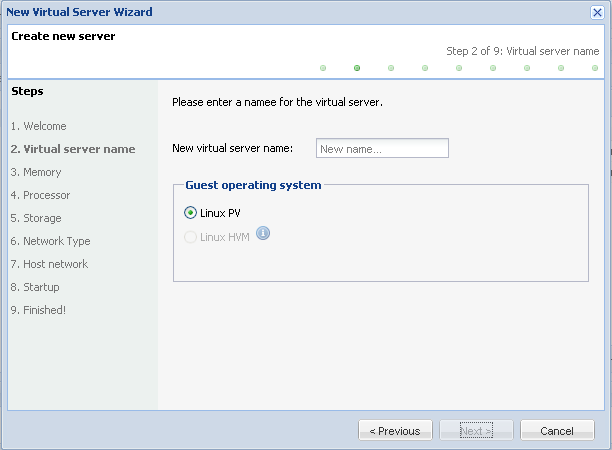
\includegraphics[scale=0.5]{screenshots/server_createwiz_name.png}
        		\caption{Add server wizard - Virtual machine name}
	        	\label{fig:server_createwiz_name}
	        	\end{center}
		\end{figure}
 
	\item[Memory:] Total assigned memory.
		\begin{figure}[H]
        		\begin{center}
		        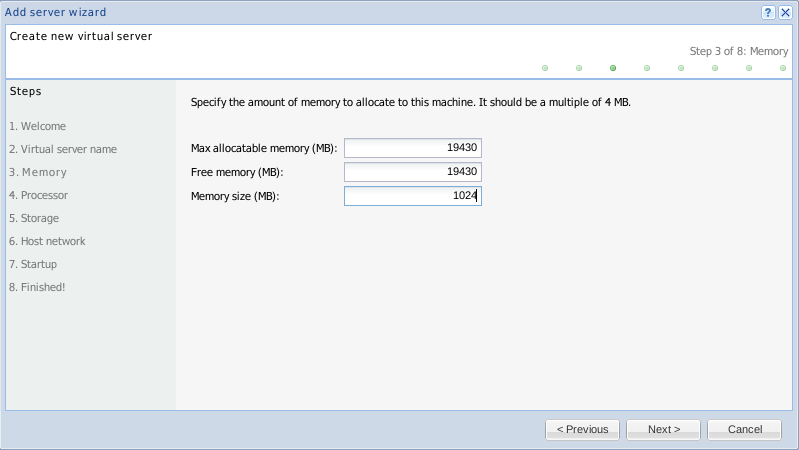
\includegraphics[scale=0.5]{screenshots/server_createwiz_memory.png}
        		\caption{Add server wizard - Memory}
	        	\label{fig:server_createwiz_memory}
	        	\end{center}
		\end{figure}

	\item[Processor:] In this stage is necessary choose the number of processor that the virtual machine will have access.
		\begin{figure}[H]
        		\begin{center}
		        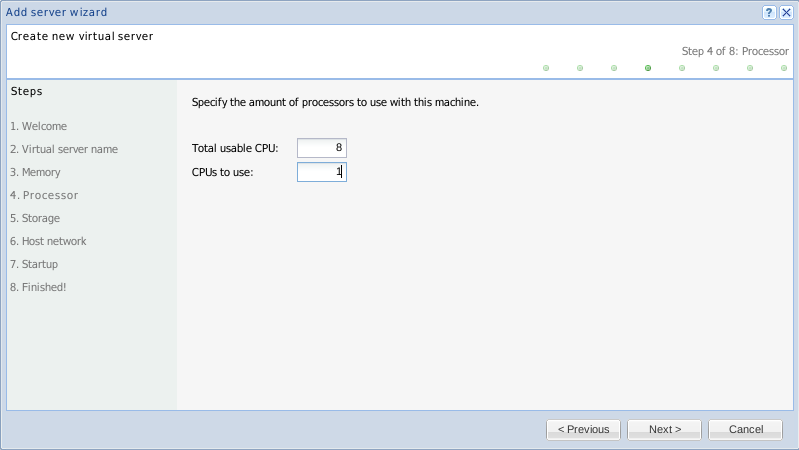
\includegraphics[scale=0.5]{screenshots/server_createwiz_processor.png}
        		\caption{Add server wizard - Processors}
		        \label{fig:server_createwiz_processor}
	        	\end{center}
		\end{figure}

	\item[Storage:] Defines the boot disk for the virtual machine. One of three options can be chosen:
\begin{itemize}
	\item use an existing logical volume/file - \emph{Existing logical volume}
	\item create a new logical volume - \emph{New logical volume}
	\item at last, a file can be created on the option \emph{New file}
\end{itemize}

        \begin{figure}[H]
        		\begin{center}
	        	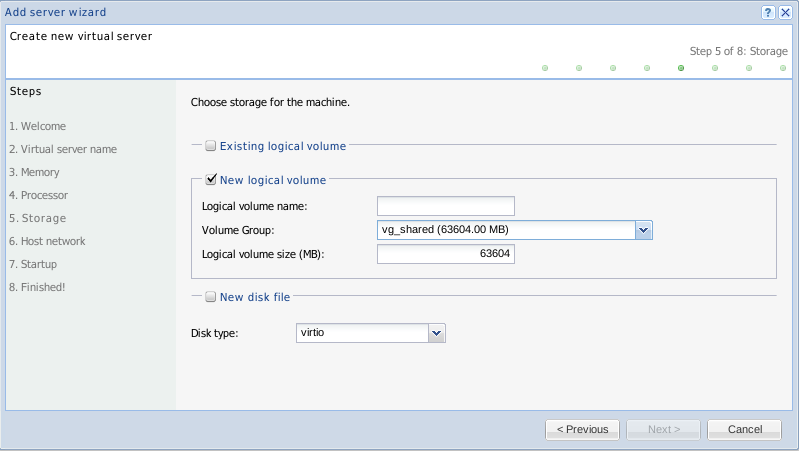
\includegraphics[scale=0.5]{screenshots/server_createwiz_storage.png}
	        	\caption{Add server wizard - Storage}
		        \label{fig:server_createwiz_storage}
        		\end{center}
		\end{figure}

		\begin{quote}
			{\large \bf Note} \\*[-.8pc]
			\underline{\hspace{6in}} \\
            If the \emph{node} does not support \emph{physical volumes} the option \emph{Existing logical volume} will be disabled.
		\end{quote}		
        
        
        \item[Host network:] Network interfaces for the server. If there are no available MAC addresses, it's possible to create new ones by pressing the \emph{MAC pool management}. Is also possible to create networks in this step using the button \emph{Add network}.
		\begin{figure}[H]
        		\begin{center}
	        	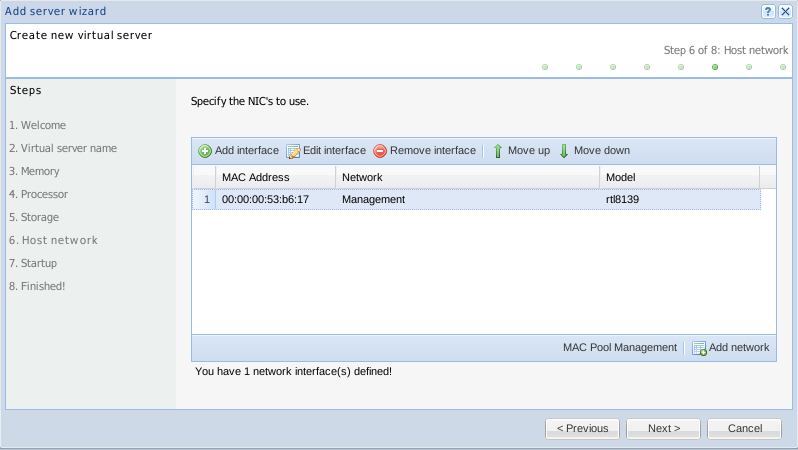
\includegraphics[scale=0.5]{screenshots/server_createwiz_hostnet.png}
	        	\caption{Add server wizard - Host network}
		        \label{fig:server_createwiz_hostnet}
        		\end{center}
		\end{figure}

        \item[Startup:] Specifies startup parameters of the virtual machine. The options at this stage vary with the type system, defined in step \emph{Virtual machine name}:		\label{sec:add_server_boot}
        \begin{itemize}
			\item \emph{Linux PV}
				\begin{itemize}
					\item Network installation. Url of the kernel.
				\end{itemize}
			\item Others
				\begin{itemize}
					\item Network Boot (PXE)
					\item CD-ROM (ISO)
				\end{itemize}
		\end{itemize}
        The figure \ref{fig:server_createwiz_startup} refers to a virtual machine options in \emph{Linux PV}.

		\begin{figure}[H]
			\begin{center}
			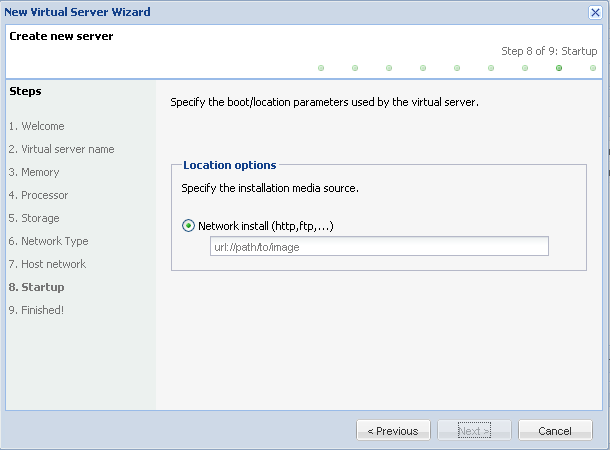
\includegraphics[scale=0.5]{screenshots/server_createwiz_startup.png}
			\caption{Add server wizard - Startup}
			\label{fig:server_createwiz_startup}
			\end{center}
		\end{figure}

	\item[Finished!] Final step of the wizard. After confirmation of the creation of the server, the data collected in previous steps are processed and sent to the virtualization server. Later in the panel \emph{servers} the virtual machine can be initiated through the option \emph{Start server}.

		\begin{figure}[H]
			\begin{center}
			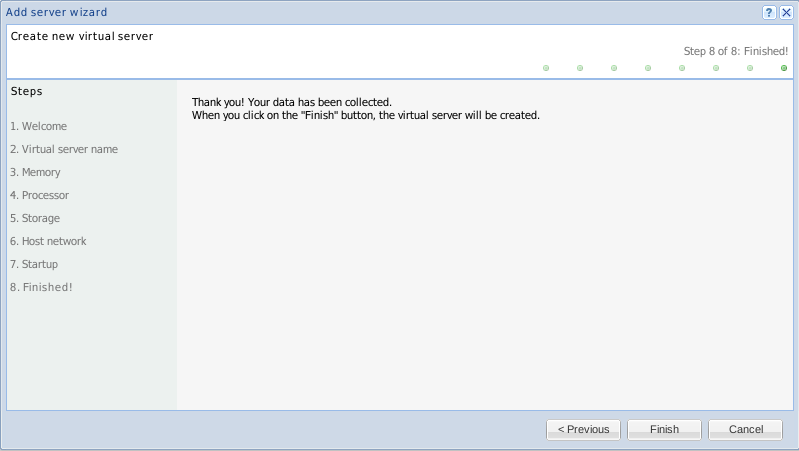
\includegraphics[scale=0.5]{screenshots/server_createwiz_finish.png}
			\caption{Add server wizard - Finished!}
			\label{fig:server_createwiz_finish}
			\end{center}
		\end{figure}

\end{description}

\subsubsection{Edit virtual machine}
\label{sec:edit_server}
To edit a server, you choose the machine you want and click on \emph{Edit server}.

    \begin{quote}
        {\large \bf Note} \\*[-.8pc]
        \underline{\hspace{6in}} \\
        If the virtual machine is running, depending on the virtual machine type and the virtualization system, some options will be disabled, it is require stop the machine in order to make the changes.
    \end{quote}

The following options are available on virtual machine configuration:
\begin{description}
	\item[General:] This allows change the name, memory, number of CPUs and number of sockets, cores and threads, operating system and boot parameters.
            The boot parameters vary depending on the virtual machine type and the virtualization system. (see Section \ref{sec:add_server_boot}).

		\begin{figure}[H]
        		\begin{center}
		        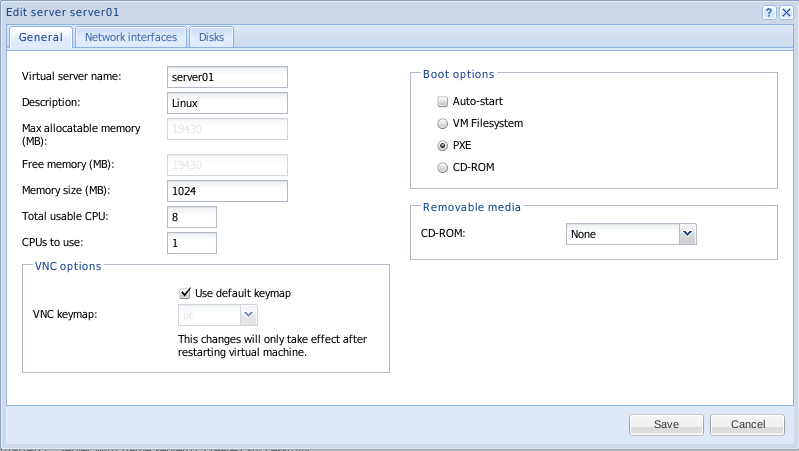
\includegraphics[scale=0.5]{screenshots/server_edit_general.png}
        		\caption{Edit server - General}
	        	\label{fig:server_edit_general}
	        	\end{center}
		\end{figure}

	\item[Network interfaces:] Add/remove interfaces. Here we can change the type of driver to use\footnote{You can only specify the driver to use if the virtual machine is HVM and KVM}.
		\begin{figure}[H]
        		\begin{center}
		        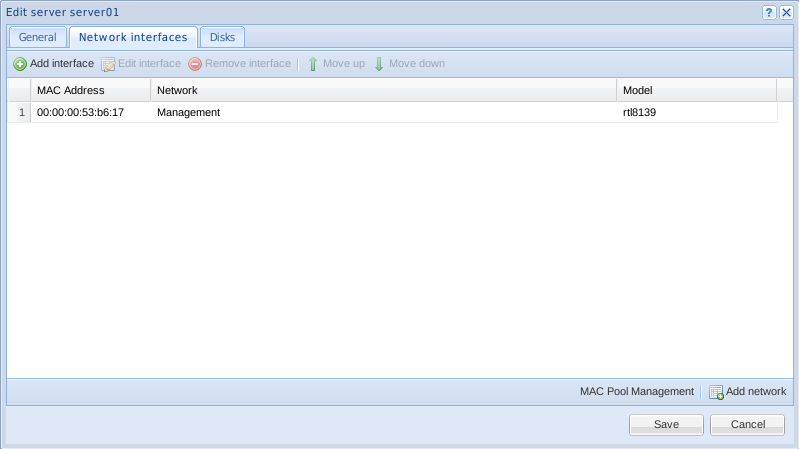
\includegraphics[scale=0.5]{screenshots/server_edit_interfaces.png}
        		\caption{Edit server - Network interfaces}
	        	\label{fig:server_edit_interfaces}
	        	\end{center}
		\end{figure}

	\item[Disks:] Add/remove machine disks. To add/remove a disk, select the desired disc and drag-n-drop between the tables.
                    
                \begin{quote}
                    {\large \bf Note} \\*[-.8pc]
                    \underline{\hspace{6in}} \\
                    The boot disk is the disk of the machine that is in first position of the table.
                \end{quote}
                    
		\begin{figure}[H]
        		\begin{center}
		        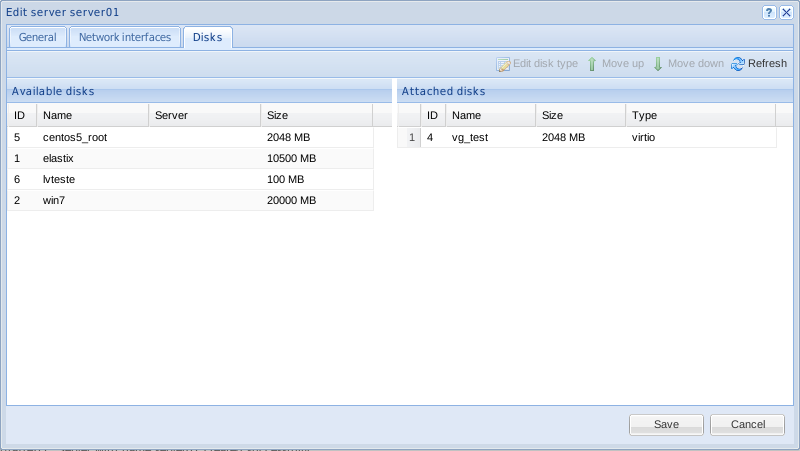
\includegraphics[scale=0.5]{screenshots/server_edit_disks.png}
        		\caption{Edit server - Disks}
		        \label{fig:server_edit_disks}
	        	\end{center}
		\end{figure}
    \item[Devices:] Attach/detach USB/PCI devices into the virtual server. A device can only be associated with one virtual server. 
                \begin{quote}
                    {\large \bf Note} \\*[-.8pc]
                    \underline{\hspace{6in}} \\
                    If the virtual server have any associated devices, it cannot be migrated/move into another node of the cluster.
                \end{quote}
    
       \begin{figure}[H]
               \begin{center}
               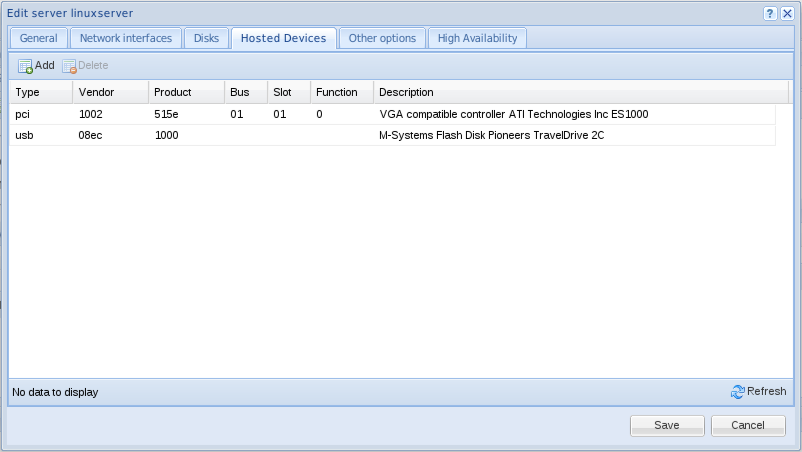
\includegraphics[scale=0.5]{screenshots/server_edit_devices.png}
               \caption{Edit server - Devices}
               \label{fig:server_edit_devices}
               \end{center}
       \end{figure}

	\item[Other options:] Lets you set VNC options like keymap and configure ACPI, APIC and PAE flags.


		\begin{figure}[H]
        		\begin{center}
		        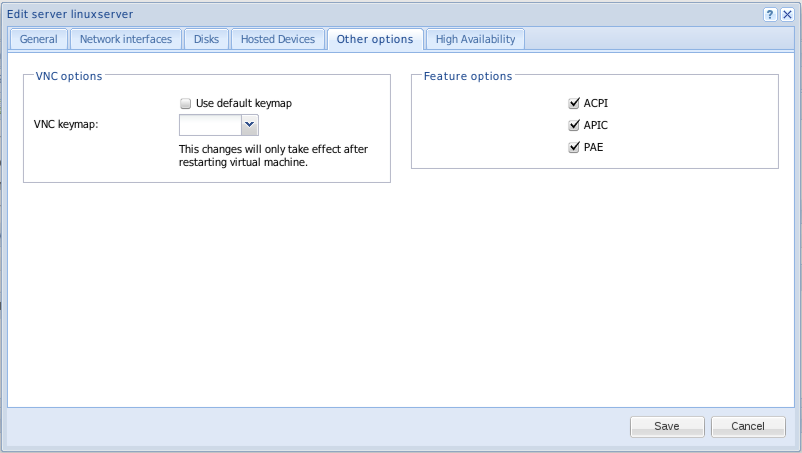
\includegraphics[scale=0.5]{screenshots/server_edit_otheroptions.png}
        		\caption{Edit server - Other options}
	        	\label{fig:server_edit_otheroptions}
	        	\end{center}
		\end{figure}

	\item[High availability:] Provides a way to configure server priority to start and to migrate and define if high availability is active on this server.


                \begin{quote}
                    {\large \bf Nota} \\*[-.8pc]
                    \underline{\hspace{6in}} \\
                    For \emph{VM High availability} we set heartbeat timeout that server should be restart if not responding.
                        This option will be available only if the guest tools are installed on virtual machine.
                \end{quote}
                    
		\begin{figure}[H]
        		\begin{center}
		        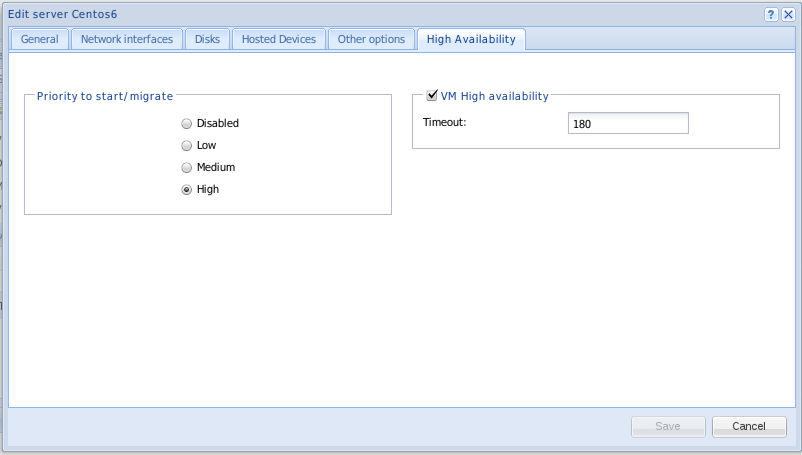
\includegraphics[scale=0.5]{screenshots/server_edit_ha.png}
        		\caption{Edit server - High availability}
	        	\label{fig:server_edit_ha}
	        	\end{center}
		\end{figure}

\end{description}



\subsubsection{Remove virtual machine}
\label{sec:remove_server}
To remove a server, choose the machine to remove and click on the button \emph{Remove server}.

The \emph{Keep disks} option keeps the hard disks connected to the machine, otherwise it will also be removed.
		
\begin{figure}[H]
	\begin{center}
	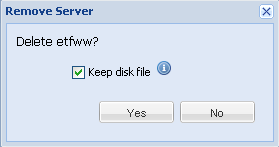
\includegraphics[scale=0.5]{screenshots/server_remove.png}
	\caption{Remove server window}
	\label{fig:server_remove}
	\end{center}
\end{figure}

\subsubsection{Connect to a virtual machine over VNC}
\label{sec:open_vnc}

Selecting a server and then clicking on button \emph{Open console} is possible to establish a VNC connection with the machine, since the machine is running.

\begin{quote}
	{\large \bf Note} \\*[-.8pc]
	\underline{\hspace{6in}} \\
    If the keyboard is mangled you can change the \emph{VNC keymap} through the option \emph{Set keymap} available in parent node context menu.
    Also, the \emph{keymap} can be defined in each server, through the option \emph{Edit server}.
\end{quote}

\subsubsection{Start/stop virtual machine}
\label{sec:start_server}

It's possible to choose between one of the following boot parameters to start the virtual machine:
\begin{description}
    \item[VM Filesystem:] Boot from the disk associated with the server.
    \item[PXE:] Boot from PXE\footnote{Only available if the type of virtual machine is not \emph{Linux PV}\label{foot:notpv}}.
    \item[Location URL:] Boot from url defined in \emph{Location}\footnote{Only available if the type of virtual machine is \emph{Linux PV}}.
	\item[CD-ROM:] Boot from a CD-ROM image\footref{foot:notpv}.
    	 
\end{description}

\begin{figure}[H]
	\begin{center}
	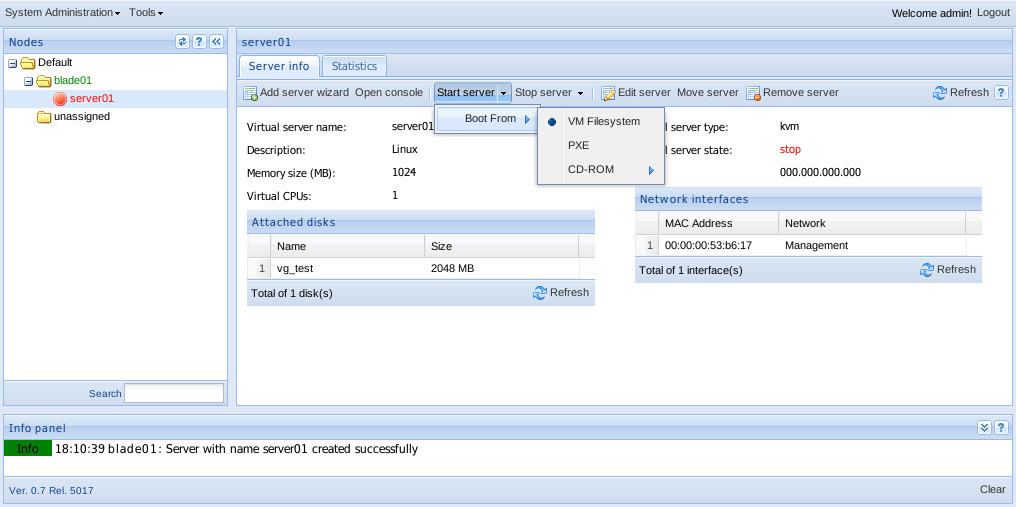
\includegraphics[scale=0.45]{screenshots/server_start.png}
	\caption{Virtual machine boot parameters}
	\label{fig:server_start}
	\end{center}
\end{figure}

It's possible to choose the option \emph{Start server} \emph{With console} to allow start the server and open console.

\subsubsection{Migrate virtual machine}
\label{sec:migrate_server}

Selecting a server and then clicking on \emph{Migrate server} you can migrate a machine from a \emph{node} to another, since they share the same storage.

\begin{figure}[H]
	\begin{center}
	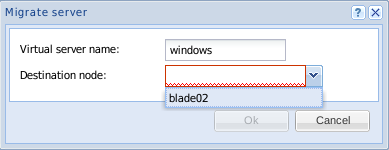
\includegraphics[scale=0.5]{screenshots/server_migrate.png}
	\caption{Virtual machine migration}
	\label{fig:server_migrate}
	\end{center}
\end{figure}

\begin{quote}
	{\large \bf Note} \\*[-.8pc]
	\underline{\hspace{6in}} \\
	This option is only available on \emph{NUXIS}.
\end{quote}

\subsubsection{Snapshots}
\label{sec:server_snapshots}

In \emph{Snapshots} we can create one \emph{snapshot} of virtual machine state, that consists on disks snapshots and, if virtual machines is running, the state of virtual machine on that moment.
It's also possible revert, remove or download of backup of one virtual machine snapshot.

\begin{figure}[H]
	\begin{center}
	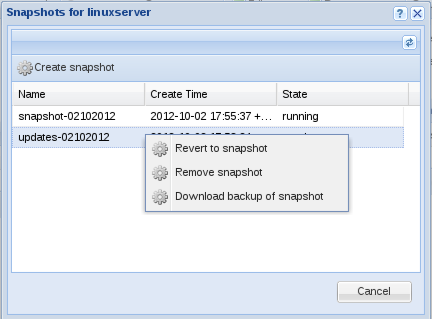
\includegraphics[scale=0.5]{screenshots/server_snapshots.png}
	\caption{Snapshots}
	\label{fig:server_snapshots}
	\end{center}
\end{figure}

\subsection{Storage}
\label{sec:storage}

The information about the existing volumes on the \emph{node} can be found on the tab \emph{Storage}.
This panel is divided into three sections:

\begin{description}
	\item[Devices -] Information about the \emph{physical volumes}\footnote{A \emph{physical volume} it's a physical device, such as a disk} and its state. Allows to do the \emph{physical volumes} administration of the \emph{node}.
	\item[Volume Groups -] List of \emph{volumes groups}\footnote{A \emph{volume group} is the aggregation of several \emph{physical volumes} in a single virtual volume} existing in the node and its associated \emph{physical volumes}. Allow \emph{volume groups} management.
	\item[Logical Volumes -] Displays information about the \emph{logical volumes}\footnote{A \emph{logical volume} it's a slice of a \emph{volume group}. It's used as a system's partition} \emph{node}. \emph{Logical volumes} administration area.
\end{description}


\begin{quote}
	{\large \bf Note} \\*[-.8pc]
	\underline{\hspace{6in}} \\
There is a special \emph{volume group}, \_\_DISK\_\_, used in the handling of files. When creating a \emph{logical volume}, this tag is used to indicate that the disk to be used is not a \emph{logical volume} but a file.
\end{quote}


\begin{figure}[H]
	\begin{center}
	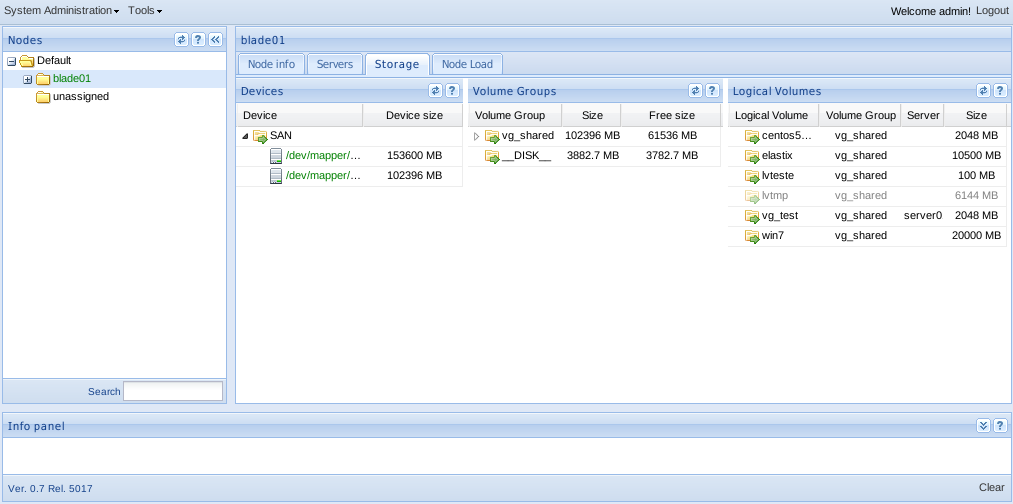
\includegraphics[scale=0.45]{screenshots/node_storage.png}
	\caption{Information about node's storage}
	\label{fig:inicial}
	\end{center}
\end{figure}

% ADMINISTRAÇÃO PHYSICAL VOLUMES

\subsubsection{Physical Volumes administration}
The \emph{physical volumes} administration consists of the following operations:
\begin{itemize}
	\item Initialize \emph{physical volume}
    \item Uninitialize \emph{physical volume}
    \item Register/Unregister \emph{physical volume}
\end{itemize}

\begin{figure}[H]
        \begin{center}
        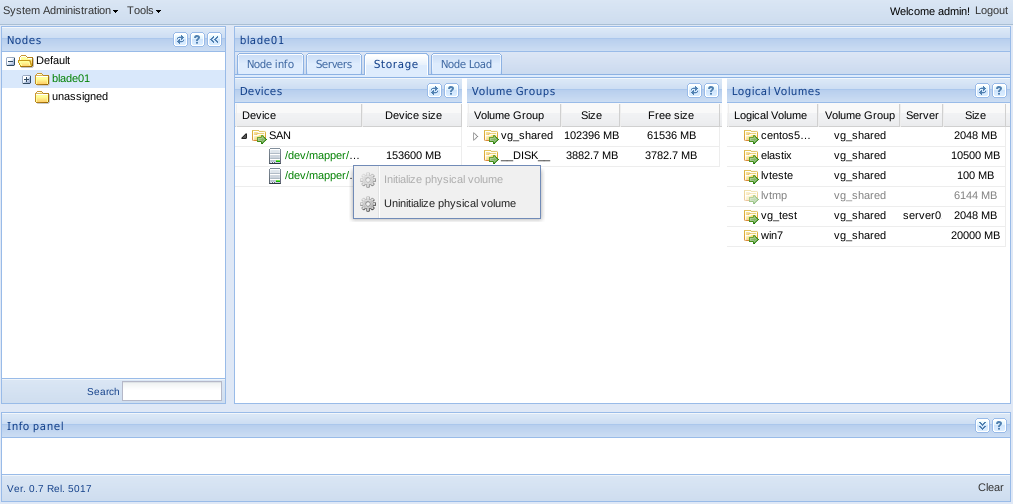
\includegraphics[scale=0.45]{screenshots/node_storage_device_ctx.png}
        \caption{Context menu of a physical volume}
        \label{fig:storage_device_ctx}
        \end{center}
\end{figure}

To initialize a \emph{physical volume}, access to the sub-context menu of the device and select \emph{Initialize physical volume}. To remove a \emph{physical volume} the operation is similar, simply select the option \emph{Uninitialize physical volume} in the context menu.

\begin{quote}
	{\large \bf Note} \\*[-.8pc]
	\underline{\hspace{6in}} \\
    The \emph{physical volume} can only be removed if it does not belong to any \emph{volume group}.
\end{quote}

\begin{figure}[H]
        \begin{center}
        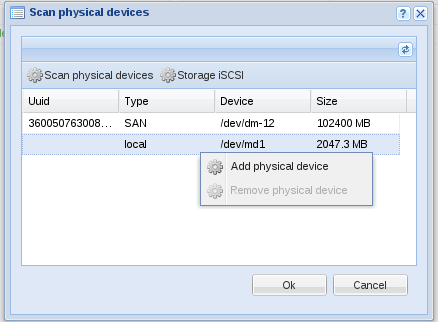
\includegraphics[scale=0.45]{screenshots/node_storage_device_search.png}
        \caption{Scan \emph{physical devices} }
        \label{fig:storage_device_search}
        \end{center}
\end{figure}

On ''Scan \emph{physical devices}'' it is possible to run a task on virtualization agent to lookup new disks and to register them on \emph{Central Management}. It is also possible to unregister the physical device on \emph{Central Management} to get it out of system management.

% ADMINISTRAÇÃO VOLUME GROUPS

\subsubsection{Volume groups administration}
In the administration of \emph{volume groups} is allowed to:
\begin{itemize}
	\item Add \emph{volume groups}
	\item Extend a \emph{volume group}
	\item Re-size a \emph{volume group}
	\item Remove a \emph{volume group}
	\item Register/Unregister \emph{volume group}
\end{itemize}

\begin{figure}[H]
        \begin{center}
        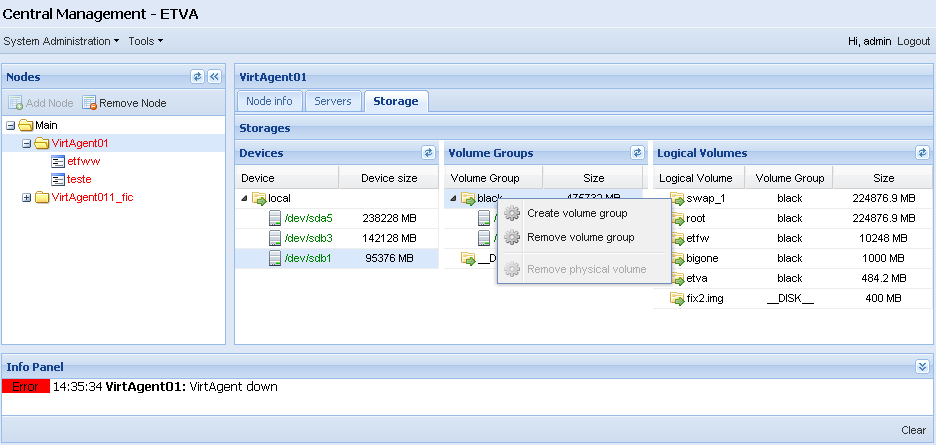
\includegraphics[scale=0.45]{screenshots/node_storage_vg_ctx.png}
        \caption{Context menu of a volume group}
        \label{fig:storage_vg_ctx}
        \end{center}
\end{figure}

To create a \emph{volume group}, access to the context menu on any \emph{volume group} and select \emph{Add volume group}.
The \emph{volume group} name should be introduced and selected one or more \emph{physical volumes} available.

A \emph{physical volume} is available when volume is not allocated to any \emph{volume group} and it's initialized.

\begin{figure}[H]
        \begin{center}
        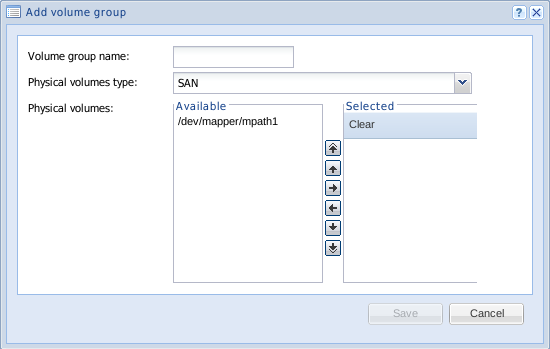
\includegraphics[scale=0.5]{screenshots/storage_vg_create.png}
        \caption{Create volume group window}
        \label{fig:storage_vg_create}
        \end{center}
\end{figure}

To extend a \emph{volume group} drag and drop a \emph{physical volume} into a \emph{volume group}.

In the removal/reduction of a \emph{volume group}, select the \emph{volume group}/\emph{physical volume} to remove and choose the corresponding option in the context menu.

\begin{quote}
	{\large \bf Note} \\*[-.8pc]
	\underline{\hspace{6in}} \\
    It's only allowed to remove a \emph{volume group} if there is no associated \emph{logical volumes}.
\end{quote}
 
\begin{figure}[H]
        \begin{center}
        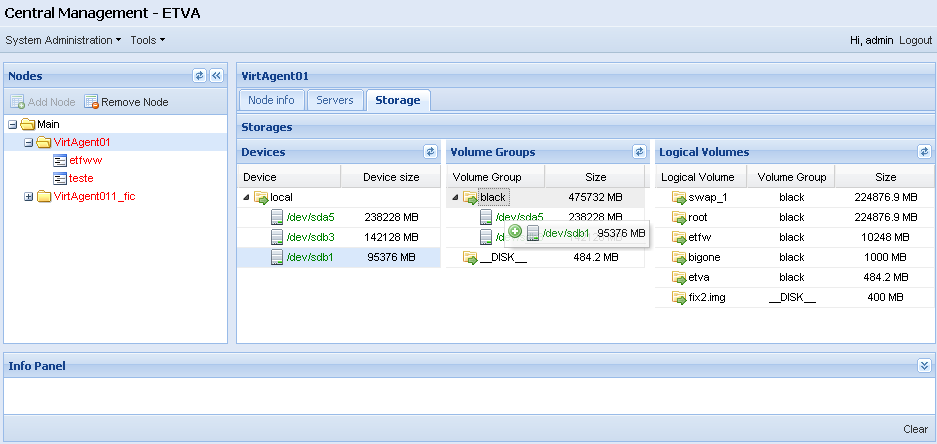
\includegraphics[scale=0.45]{screenshots/storage_vg_extend.png}
        \caption{Volume group extension}
        \label{fig:storage_vg_extend}
        \end{center}
\end{figure}

On Figure \ref{fig:storage_vg_extend} we extend a \emph{volume group} with a new \emph{physival volume}.

\begin{figure}[H]
        \begin{center}
        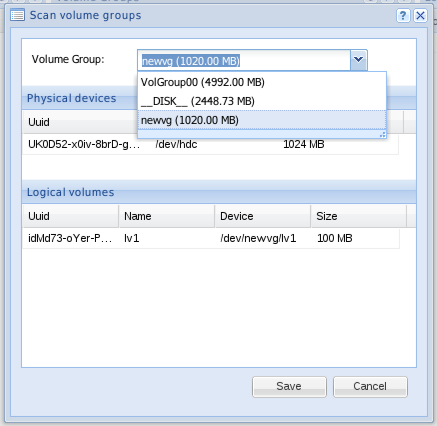
\includegraphics[scale=0.45]{screenshots/node_storage_vg_search.png}
        \caption{Scan \emph{volume groups}}
        \label{fig:storage_vg_search}
        \end{center}
\end{figure}

On ''Scan \emph{volume groups}'', it is possible to get \emph{volume groups} from virtualization agent and register them on \emph{Central Management}.
Is is also possible to unregister the \emph{volume group} on \emph{Central Management} to get it out of system management.

% ADMINISTRAÇÃO LOGICAL VOLUMES

\subsubsection{Logical volumes administration}

The operations available on the \emph{logical volumes} are:
\begin{itemize}
	\item Create a \emph{logical volume}
	\item Resize a \emph{logical volume}
	\item Remove a \emph{logical volume}
	\item Register/Unregister \emph{logical volume}
    \item Clone \emph{logical volume}
    \item Convert \emph{logical volume}
\end{itemize}

\begin{figure}[H]
        \begin{center}
        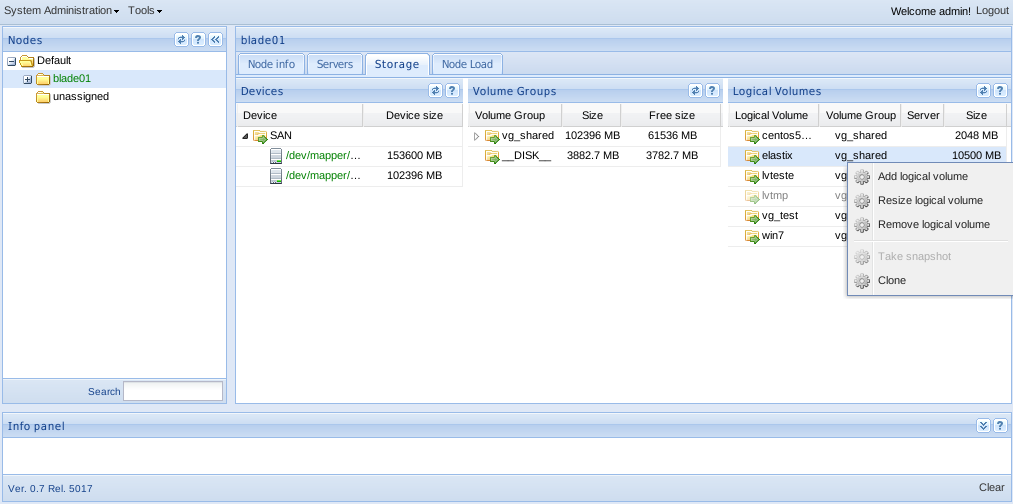
\includegraphics[scale=0.45]{screenshots/node_storage_lv_ctx.png}
        \caption{Logical volume context menu}
        \label{fig:storage_lv_ctx}
        \end{center}
\end{figure}

To create a new \emph{logical volume}, we access the context menu (over any \emph{logical volume}, and select the option \emph{Add logical volume}.

The pretended name should be introduced in the creation window form, such as the \emph{volume group} size. Note that the size should not exceed the \emph{volume group} available size.
It's also possible define the format of disk (raw, cow2,qcow,cow and vmdk - raw by default) and percentage of \emph{snapshot} usage.

\begin{figure}[H]
        \begin{center}
        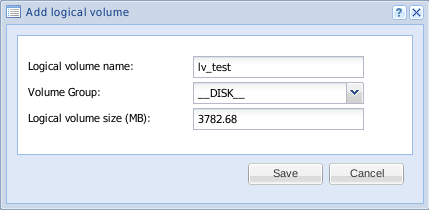
\includegraphics[scale=0.5]{screenshots/storage_lv_create.png}
        \caption{Create a new logical volume window}
        \label{fig:storage_lv_create}
        \end{center}
\end{figure}

To resize a \emph{logical volume}, select and access into the context menu. The we can find the option \emph{Resize logical volume}, that allow us to increase/reduce the \emph{logical volume} size.

\begin{quote}
	{\large \bf Note} \\*[-.8pc]
	\underline{\hspace{6in}} \\
    By reducing the size of a \emph{logical volume} could make existing data unusable. It is your responsibility to check that it is affordable/secure resizing the \emph{logical volume} without affecting the data.
\end{quote}


\begin{figure}[H]
        \begin{center}
        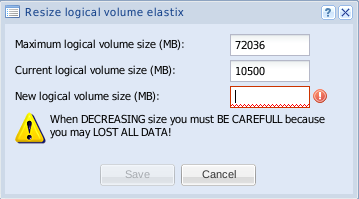
\includegraphics[scale=0.5]{screenshots/storage_lv_resize.png}
        \caption{Resize of a volume group}
        \label{fig:storage_lv_resize}
        \end{center}
\end{figure}

To remove a \emph{logical volume}, access the context menu and select the option \emph{Remove logical volume}. The \emph{logical volume} will be removed if it's not assigned to any virtual machine. To verify if is in use you may pass the mouse over the \emph{logical volume} and observe the information contained in the \emph{tooltip}.

We have the operation to clone one \emph{logical volume}, if \emph{volume group} have free space to do the copy.
And we can convert the disks format to one of the formats (raw, qcow2, qcow, cow and vmdk).

\begin{figure}[H]
        \begin{center}
        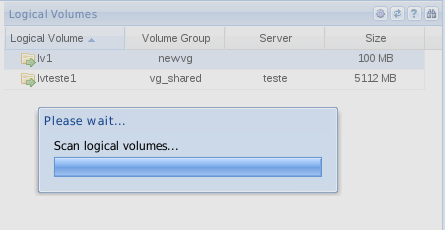
\includegraphics[scale=0.45]{screenshots/node_storage_lv_search.png}
        \caption{Scan \emph{logical volumes}}
        \label{fig:storage_lv_search}
        \end{center}
\end{figure}

On ''Scan \emph{logical volumes}'' it synchronizes \emph{logical volumes} that are on virtualization agent and they are not registered on \emph{Central Management}.
It is may be possible that exist \emph{logical volumes} that are registered on \emph{Central Management} but really don't exist for some reason.
In this cases, it is possible remove the register from the system and get the \emph{logical volumes} synchronized with ''Scan \emph{logical volumes}''.

\subsection{Node Load}
\label{sec:nodeload}
In the \emph{Node Load} panel, we can find information about the node's load. In Figure \ref{fig:node_load}, we can see the load information of the node in a hour range.



\begin{figure}[H]
        \begin{center}
        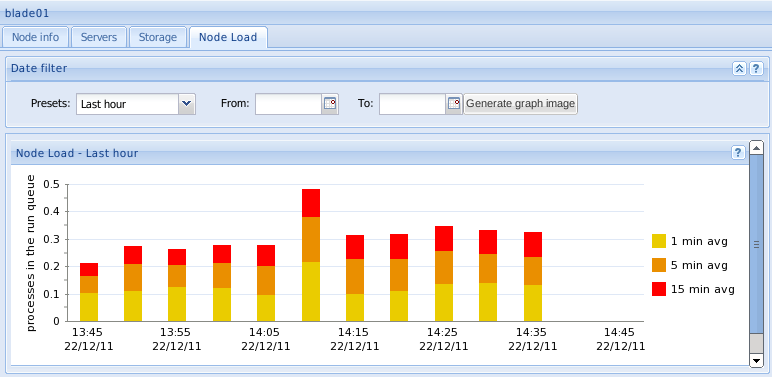
\includegraphics[scale=0.6]{screenshots/node_load.png}
        \caption{Node load}
        \label{fig:node_load}
        \end{center}
\end{figure}

In this panel we can also view the data by intervals:
\begin{itemize}
	\item Last hour
	\item Last 2 hours
	\item Last 24 hours
	\item Last week
\end{itemize}
To view other time intervals use the option \emph{Generate graph image}. The image is generated as shown in figure \ref{fig:server_stats_nodeLoadRange}.

\begin{figure}[H]
	\begin{center}
	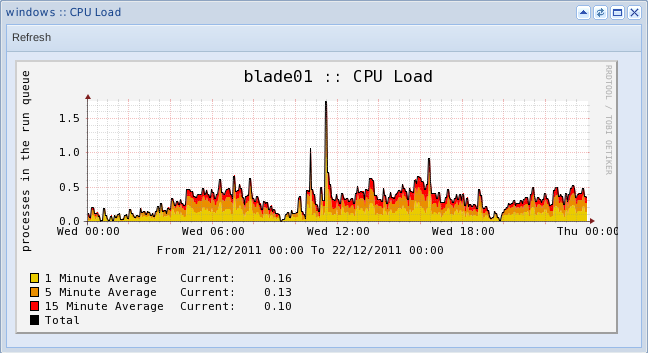
\includegraphics[scale=0.6]{screenshots/server_stats_nodeLoadRange.png}
	\caption{Node usage statistics - CPU load}
	\label{fig:server_stats_nodeLoadRange}
	\end{center}
\end{figure}

\subsection{Shutdown node}
\label{sub:shutdown_node}
Through the Central Management interface we can power off a physical node. To do so do the following steps:

\begin{itemize}
\item On the left panel, select the desired node. Then access to it's context menu;
\item Press the option \textit{Shutdown}.
\end{itemize}

\begin{quote}
    {\large \bf Note} \\*[-.8pc]
    \underline{\hspace{6in}} \\
    During the procedure, all node's virtual servers will also turned off.
\end{quote}


\begin{figure}[H]
        \begin{center}
        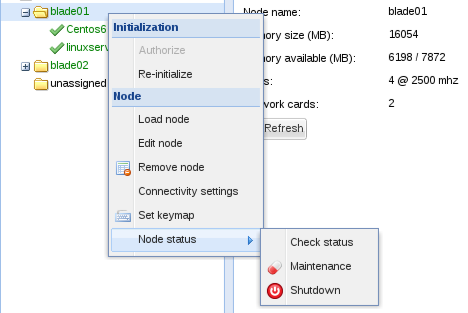
\includegraphics[scale=0.45]{screenshots/shutdownnode.png}
        \caption{Shutting down a node}
        \label{fig:storage_lv_ctx}
        \end{center}
\end{figure}


\pagebreak

\section{Virtual machine}
\label{sec:server}
In the nodes pane we can select the virtual machine on which we intend to perform operations such as:

\begin{itemize}
        \item Manage the virtual machine
        \item View usage statistics 
        \item Manage \emph{Management Agent} services
\end{itemize}

\subsection{Server information}
In \emph{Information Server} we can see the state of the virtual machine and, among other information, the state of the \emph{Management Agent}.
In addition to displaying information, this panel lets you perform the following operations:

\begin{itemize}
	\item Add a virtual machine (see Section \ref{sec:add_server})
    \item Edit a virtual machine (see Section \ref{sec:edit_server})
	\item Remove virtual machine (see Section \ref{sec:remove_server})
	\item Open a virtual machine in a VNC console (see Section \ref{sec:open_vnc})
	\item Start/stop virtual machine (see Section \ref{sec:start_server})
    \item Migrate a virtual machine (see Section \ref{sec:migrate_server})
    \item Snapshots (see Section \ref{sec:server_snapshots})
\end{itemize}

\begin{figure}[H]
	\begin{center}
	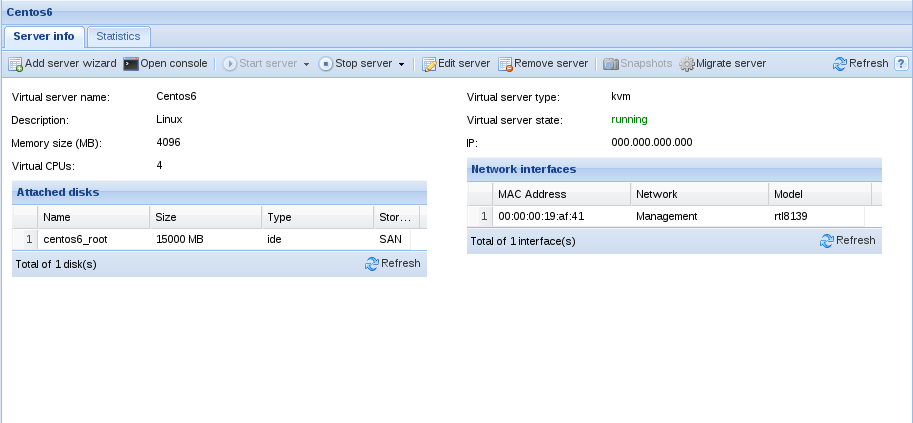
\includegraphics[scale=0.45]{screenshots/server_info.png}
	\caption{Information about the virtual machine}
	\label{fig:server_info}
	\end{center}
\end{figure}

\subsection{Statistics}
In \emph{statistics} tab it's possible to see, graphically, information about:
\begin{itemize}
	\item Cpu Usage (Figure \ref{fig:vm_cpuload})
	\item Networks (Figure \ref{fig:vm_interfaces})
	\item Memory Usage (Figure \ref{fig:vm_mem})
	\item Disk (Figure \ref{fig:vm_disk_io})
\end{itemize}


\begin{figure}[H]
	\begin{center}
	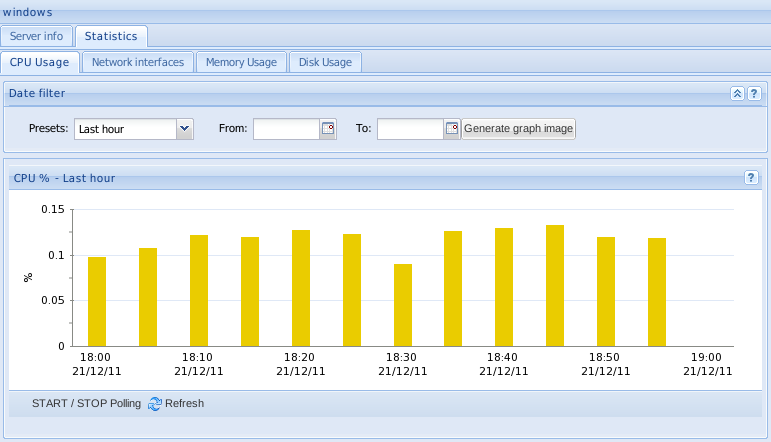
\includegraphics[scale=0.45]{screenshots/vm_cpuload.png}
	\caption{Virtual machine cpu load}
	\label{fig:vm_cpuload}
	\end{center}
\end{figure}

\begin{figure}[H]
	\begin{center}
	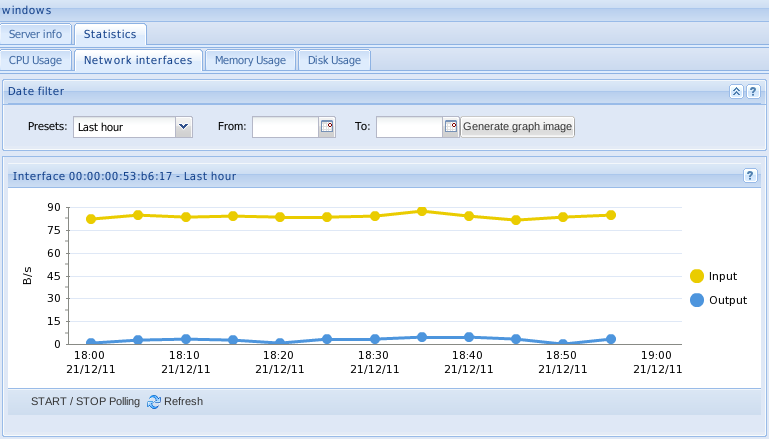
\includegraphics[scale=0.45]{screenshots/vm_interfaces.png}
	\caption{Virtual machine network interfaces}
	\label{fig:vm_interfaces}
	\end{center}
\end{figure}

\begin{figure}[H]
	\begin{center}
	\includegraphics[scale=0.45]{screenshots/vm_mem.png}
	\caption{Virtual machine memory usage}
	\label{fig:vm_mem}
	\end{center}
\end{figure}

\begin{figure}[H]
	\begin{center}
	\includegraphics[scale=0.45]{screenshots/vm_disk_io.png}
	\caption{Virtual machine disk input/output}
	\label{fig:vm_disk_io}
	\end{center}
\end{figure}

In each of these panels we can view the data by pre-set intervals. For more information see Section \ref{sec:nodeload}.

\subsection{Services}
In \emph{Services} tab panel, we can configure the available services on the corresponding management agent.

\subsection{Virtio drivers}
The virtio drivers facilitate communication between the operating system that runs the virtual machine, and the various hardware components. These components are the network devices and storage units - disks. As the use of the virtio drivers increases the overall system, its installation is recommended.

If the virtual machine's operating system is a complete Linux distribution whose kernel is a version less than 2.6.25, the virtio is supported without the need to follow any procedure to install the drivers. To take advantage of, simply select the driver tab virtio \textit{Network Interfaces} and \textit{Disks} on \textit{server edit} window.

The requirements for the use of the virtio drivers can be found at:

http://wiki.libvirt.org/page/Virtio

\subsubsection*{Installation on windows virtual machines}

Download the iso with the drivers, available at:

http://alt.fedoraproject.org/pub/alt/virtio-win/latest/images/bin/.

Upload iso with the drivers - more information in Section \ref{sec:iso_manager}. \textit{Tools}, \textit{ISO Manager}, \textit{upload applet}, select the file and upload. The file should appear in the list of ISOs.

Then select the server where you want to install the drivers, and choose the \textit{Edit server}. Choose the ISO image with the drivers as shown in Figure \ref{fig:virtio4}. Go to the tab \textit{Disk} and assign a new volume, choosing the virtio driver - Figure \ref{fig:virtio7}.

\begin{figure}[H]
	\begin{center}
	\includegraphics[scale=0.5]{screenshots/virtio/virtio_4.png}
	\caption{Driver's - iso selection}
	\label{fig:virtio4}
	\end{center}
\end{figure}

\begin{figure}[H]
	\begin{center}
	\includegraphics[scale=0.5]{screenshots/virtio/virtio_7.png}
	\caption{Set logical volume (drivers virtio)}
	\label{fig:virtio7}
	\end{center}
\end{figure}

Set the startup disk server as shown in Figure \ref{fig:virtio5}.

\begin{figure}[H]
	\begin{center}
	\includegraphics[scale=0.5]{screenshots/virtio/virtio_5.png}
	\caption{Set the startup disk}
	\label{fig:virtio5}
	\end{center}
\end{figure}

With Windows running, go to device manager. Note that the added logical volume appears as shown in Figure \ref{fig:virtio10}.

Then select the \textit{Update Driver Software}, \textit{Browse my computer for driver software}, indicate where is the drivers (in the virtual CD drive), completing the installation procedure.

\begin{figure}[H]
	\begin{center}
	\includegraphics[scale=0.5]{screenshots/virtio/virtio_10.png}
	\caption{Windows - driver update}
	\label{fig:virtio10}
	\end{center}
\end{figure}

Stop the virtual machine and edit the settings by changing the main driver of the logical volume where you installed the operating system - Figure \ref{fig:virtio16}.

\begin{figure}[H]
	\begin{center}
	\includegraphics[scale=0.5]{screenshots/virtio/virtio_16.png}
	\caption{Change the disk driver to virtio}
	\label{fig:virtio16}
	\end{center}
\end{figure}

\section{Tools}

In menu \emph{Tools} we can access the folloing options:
\begin{itemize}
\item Import OVF
\item Export OVF
\item ISO Manager
\item Node agent monitor
\item System events' log
\end{itemize}

\subsection{Import OVF}
This tool allows you to import virtual machines in OVF format (\emph{Open Virtualization Format}).

\begin{figure}[H]
	\begin{center}
	\includegraphics[scale=0.5]{screenshots/ovf_import.png}
	\caption{OVF import wizard - Welcome}
	\label{fig:ovf_import_wiz}
	\end{center}
\end{figure}
The OVF import wizard is constituted by the following stages:

\begin{description}
	\item[Source OVF file:] In this stage we define the OVF file URL (see Figure \ref{fig:ovf_import_file}).
		
        \begin{quote}
            {\large \bf Note} \\*[-.8pc]
            \underline{\hspace{6in}} \\
            The CM must have HTTP access to the specified URL.
        \end{quote}

        \begin{figure}[H]
            \begin{center}
            \includegraphics[scale=0.5]{screenshots/ovf_import_file.png}
            \caption{OVF import wizard - Source OVF file}
            \label{fig:ovf_import_file}
            \end{center}
        \end{figure}

	\item[OVF details:] OVF file details. Provides information about the product, version, total size of the files referenced by the OVF, if available.
		\begin{figure}[H]
            \begin{center}
            \includegraphics[scale=0.5]{screenshots/ovf_import_resume.png}
            \caption{OVF import wizard - OVF details}
            \label{fig:ovf_import_resume}
            \end{center}
        \end{figure}

    \item[License:] If specified in the OVF file, this step will come with the EULA. Otherwise, this step is omitted.
		\begin{figure}[H]
            \begin{center}
            \includegraphics[scale=0.5]{screenshots/ovf_import_eula.png}
            \caption{OVF import wizard - License}
            \label{fig:ovf_import_eula}
            \end{center}
        \end{figure}

    \item[Name and location:] This step defines the virtual machine name, the destination node and the type of operating system. The operating system options vary depending on the specification of the node:
		\begin{itemize}
			\item with XEN and hardware hardware support:
			\begin{itemize}
				\item Linux PV
				\item Linux HVM
				\item Windows
			\end{itemize}
 			\item with XEN and without the hardware support:
			\begin{itemize}
				\item Linux PV
			\end{itemize}
 			\item with KVM
			\begin{itemize}
				\item Linux
				\item Windows
			\end{itemize}
		\end{itemize}

        \begin{figure}[H]
            \begin{center}
            \includegraphics[scale=0.5]{screenshots/ovf_import_name.png}
            \caption{OVF import wizard - Name and location}
            \label{fig:ovf_import_name}
            \end{center}
        \end{figure}
        Before proceeding to the next step, the wizard checks if the disks' drivers and network interfaces mentioned in the OVF are supported by the chosen virtualization server.

        The supported drivers by XEN machines, with or without hardware virtualization, are: IDE, SCSI and xen and in machines with KVM drivers are: ide, virtio and scsi.

        The supported network card drivers for HVM and KVM machines are: e1000, virtio and rtl8139. On a XEN machine without hardware virtualization support, no drivers can be used.

        If the selected virtualization server does not to support the drivers mentioned, the OVF import can not be performed.


    \item[Storage:] This step is carried out mapping of disks in the node. You can specify the name of the \emph{logical volume} and define the its \emph{volume group}.
         It is required that all disks are mapped to proceed to the next step.        
		\begin{figure}[H]
            \begin{center}
            \includegraphics[scale=0.5]{screenshots/ovf_import_storage.png}
            \caption{OVF import wizard - Storage}
            \label{fig:ovf_import_storage}
            \end{center}
        \end{figure}    

    \item[Network interfaces:] In this stage we map the network interfaces. You can specify new network interfaces.
         It is necessary that all the network interfaces are mapped to proceed to the next step.
		\begin{figure}[H]
            \begin{center}
            \includegraphics[scale=0.5]{screenshots/ovf_import_networks.png}
            \caption{OVF import wizard - Network interfaces}
            \label{fig:ovf_import_networks}
            \end{center}
        \end{figure}

    \item[Finished!:] Final step of the wizard. After confirmation of the import of virtual machine, the collected data in previous steps are processed and sent to the virtualization server. Later in the panel \emph{server} the virtual machine can be initiated through the option \emph{Start server}.
		\begin{figure}[H]
			\begin{center}
			\includegraphics[scale=0.5]{screenshots/ovf_import_finish.png}
            \caption{OVF import wizard - Finished!}
			\label{fig:ovf_import_finish}
			\end{center}
		\end{figure}

\end{description}

\subsection{Export OVF}
This tool allows you to export virtual machines in OVF format (\emph{Open Virtualization Format}).
The generated file will be in the OVA format (\emph{Open Virtualization Archive}).

\begin{quote}
	{\large \bf Note} \\*[-.8pc]
	\underline{\hspace{6in}} \\
    The virtual machine to export needs to be stopped to perform the export.
\end{quote}

\begin{figure}[H]
	\begin{center}
	\includegraphics[scale=0.5]{screenshots/ovf_export.png}
	\caption{OVF export window}
	\label{fig:ovf_export}
	\end{center}
\end{figure}


\subsection{ISO manager}
\label{sec:iso_manager}
this tool allows you to manage the images that will be available for use in virtual machines.
The files will be used later for mounting virtual machine's \emph{CD-ROM} unit.

\begin{figure}[H]
	\begin{center}
	\includegraphics[scale=0.5]{screenshots/iso_manager.png}
	\caption{Iso management panel}
	\label{fig:iso_manager}
	\end{center}
\end{figure}

The supported operations are:
\begin{itemize}
\item Upload of multiple files
\item Download of files
\item Rename files
\item Delete files
\end{itemize}


\begin{quote}
	{\large \bf Note} \\*[-.8pc]
	\underline{\hspace{6in}} \\
    Changes to existing images that are set at boot from CD-ROM of any virtual machine, will not be reflected automatically. The user must check if the mounted image on the CD-ROM unit is still valid.
\end{quote}

\subsection{Nodes' agent monitor}
This tool is for real-time communication testing of the multiple nodes of the CM. Verification is done periodically.
To stop checking close the pop up that appears when activating the tool.

\subsection{System events log}
\label{sec:system_event_reg}

In \emph{System events log} menu it's possible to see the changes made by user interaction.

\begin{figure}[H]
	\begin{center}
	\includegraphics[scale=0.4]{screenshots/events_log.png}
	\caption{System events log window}
	\label{fig:events_log}
	\end{center}
\end{figure}

The event log messages can be filtered by three message types:
\begin{itemize}
    \item {\bf Debug} - Displays all messages. Aggregate levels \emph{Info} and \emph{Error}
    \item {\bf Info} - Messages with information on events that have been successful
    \item {\bf Error} - Messages with information on events that haven't been successful
\end{itemize}

\section{System administration}
\label{sec:first_time_wizard}
In the \emph{System administration} menu it's possible we can access to:
\begin{itemize}
\item One-time setup wizard
\opt{etvm}{
    \item Cluster setup wizard
}
\item Change preferences
\item Users' and permissions' administration
\end{itemize}

\subsection{One time set wizard}
The initialization setup wizard gathers the set of operations to be carried out on first access to the CM. Lets you make a quick system configuration.

The setup wizard, as shown in Figure \ref{fig:first_time_wizard}, consists in the following steps:

\begin{itemize}
	\item Default password change
	\item MAC pool generation
    \item System preferences
	\item Network setup
\end{itemize}

\begin{figure}[H]
        \begin{center}
        \includegraphics[scale=0.7]{screenshots/first_time_wizard.png}
        \caption{One time setup wizard}
        \label{fig:first_time_wizard}
        \end{center}
\end{figure}

\begin{quote}
	{\large \bf Note} \\*[-.8pc]
	\underline{\hspace{6in}} \\
	On version \emph{NUXIS}, the network configuration step is omitted.
\end{quote}

\opt{etvm}{
\subsection{Virtual cluster management}
When we select one of the tree nodes that appears in the left panel, is shown in the right panel its context panels - Figure \ref{fig:cluster-context}. In them you can manage the networks and shared storage volumes, always in the context of the selected virtual datacenter (cluster).

\begin{figure}[H]
        \begin{center}
        \includegraphics[scale=0.6]{screenshots/cluster-context.png}
        \caption{Cluster management panels}
        \label{fig:cluster-context}
        \end{center}
\end{figure}


\subsubsection{Virtual cluster setup wizard}
The cluster setup wizard enables the definition of a new cluster of nodes. Each cluster has its own networks, and shared storage volumes \footnote{Option only available in version \emph{NUXIS}}.

To open the wizard select \textit{System Administration} followed by the option \textit{Cluster setup wizard}. Then you will see the setup window, which requires the following configuration steps (Figure \ref{fig:cluster_config}):

\begin{enumerate}
	\item Set the name of the data center, which can be changed later
	\item Define the networks that nodes are going to have access. For more information see Section \ref{sub:network}
\end{enumerate}

\begin{figure}[H]
        \begin{center}
        \includegraphics[scale=0.6]{screenshots/cluster_config.png}
        \caption{Virtual cluster setup wizard}
        \label{fig:cluster_config}
        \end{center}
\end{figure}

\subsubsection{Moving a node between datacenters}
You can move nodes between existing data centers. For this purpose it is necessary that the node has not been authorized, i.e., by selecting the option \emph{Authorize} in the node's context menu - see Figure \ref{fig:cluster-move}).

To move, drag and drop the node to the desired target (datacenter).
\begin{figure}[H]
        \begin{center}
        \includegraphics[scale=0.6]{screenshots/cluster-move.png}
        \caption{Move nodes between clusters (\emph{NUXIS} version)}
        \label{fig:cluster-move}
        \end{center}
\end{figure}

\subsubsection{Authorize node}
When a new node is added, it appears in the left pane with the text color in blue. In this case, in order to manage through the \textit{Central management}, you must authorize it.

To proceed with the authorization, select the desired node and access into its context menu (right click on the mouse button). Then select \textit{Authorize}. The Figure \ref{fig:cluster-auth} and \ref{fig:cluster-auth} illustrate the process.

\begin{figure}[H]
        \begin{center}
        \includegraphics[scale=0.6]{screenshots/cluster-auth.png}
        \caption{Node authorization}
        \label{fig:cluster-auth}
        \end{center}
\end{figure}

\begin{figure}[H]
        \begin{center}
        \includegraphics[scale=0.6]{screenshots/cluster-auth1.png}
        \caption{Authorize node - performing operation}
        \label{fig:cluster-auth1}
        \end{center}
\end{figure}
In the authorization process, the \textit{Central Management} checks if the node has the same vision of shared storage volumes as the other cluster nodes. If an error occur, check the system's event log - see Section \ref{sec:system_event_reg}.
}% End of the section of NUXIS

\subsection{System Preferences}
By accessing the system references you can set some parameters. 
In the general panel you can specify the default VNC keymap to access virtual machines as well as define the duration of the event logs of the system.
 
\begin{figure}[H]
        \begin{center}
        \includegraphics[scale=0.5]{screenshots/preferences_general.png}
        \caption{System preferences window - General panel}
        \label{fig:preferences_general}
        \end{center}
\end{figure}

In the connectivity tab you're allowed to change the CM IP address and for the LAN network (only available in \emph{NUXIS} version. In the \emph{NUXIS} version you are only allowed to change the CM IP.

\begin{figure}[H]
        \begin{center}
        \includegraphics[scale=0.5]{screenshots/preferences_conn.png}
        \caption{System preferences window - Connectivity tab}
        \label{fig:preferences_conn}
        \end{center}
\end{figure}

\subsection{Users, groups and permission administration}
The administration menu is available to the super users the system, and can be found on the top bar (then tools), in \textit{Users' and permissions' administration}.

When we select this option, a window with three following tabs is open:
\begin{itemize}
	\item \textit{User management};
	\item \textit{Group management};
	\item \textit{Permission management}.
\end{itemize}

The image \ref{fig:user_admin} illustrates the window that appears. In this window you can set the necessary permissions. Users can be created to access the management interface, and assigned access permissions on virtual machine level, or on cluster cluster level.

To facilitate the assignment of permissions you can set groups. For example, one group can have several associated permissions, and can be assigned to multiple users. This makes adding/removing a set of permissions to users easier.


\begin{figure}[H]
        \begin{center}
        \includegraphics[scale=0.4]{screenshots/permissions/user.png}
        \caption{Users' and permissions' administration}
        \label{fig:user_admin}
        \end{center}
\end{figure}

In addition, you have another way to assign permissions and/or groups, right clicking the mouse on the desired node/server, as stated on Figures \ref{fig:context_dc}, \ref{fig:context_server} and \ref{fig:server_window}.

\begin{figure}[H]
        \begin{center}
        \includegraphics[scale=0.5]{screenshots/permissions/context_dc.png}
        \caption{Permission option in node's context}
        \label{fig:context_dc}
        \end{center}
\end{figure}

\begin{figure}[H]
        \begin{center}
        \includegraphics[scale=0.5]{screenshots/permissions/context_server.png}
        \caption{Permission option in server's context}
        \label{fig:context_server}
        \end{center}
\end{figure}

\begin{figure}[H]
        \begin{center}
        \includegraphics[scale=0.5]{screenshots/permissions/server_window.png}
        \caption{Changing servers' access permissions}
        \label{fig:server_window}
        \end{center}
\end{figure}

\begin{quote}
	{\large \bf Note} \\*[-.8pc]
	\underline{\hspace{6in}} \\    
    In \emph{Manage groups} it's not possible to remove the group with ID=1 (system reserved).
\end{quote}

\opt{etvm}{
    \subsection{Shutdown Central Management}
    To turn off Central Management we must access the \textit{System Administration} menu, and choose the \textit{Shutdown Central Management} option. Then answer yes to the confirmation question.

\begin{quote}
    {\large \bf Note} \\*[-.8pc]
    \underline{\hspace{6in}} \\
    Shutting down Central Management will also terminate any existing virtual machines.
\end{quote}
}

\opt{etva}{
    \subsection{Shutdown appliance}
    There are two methods to turn off the \textit{ETVA appliance}. The first method is through the management interface, executing the steps below:

    \begin{itemize}
    \item Access the Central Management interface
    \item Select the desired node and access it's context menu
    \item Press the option \textit{Shutdown}. This option will also turn off any virtual machines of the node.
    \end{itemize}

    The other way of shutting down is using the appliance's display buttons (see Figure \ref{fig:app_display}).

    \begin{itemize}
    \item Select MENU;
    \item Search the option SHUTDOWN;
    \item Press the ENTER button.
    \end{itemize}

    \begin{figure}[H]
        \begin{center}
        \includegraphics[scale=0.3]{screenshots/appliancedisplay.jpg}
        \caption{ETVA display and buttons}
        \label{fig:app_display}
        \end{center}
    \end{figure}
}


\pagebreak
